\chapter{Modelado y Experimentación}
\label{cap:modelado}

Una vez construido y preparado el conjunto de datos de 20,000 muestras, el ciclo de vida de la metodología \textbf{Komorebi} \cite{verges_como_2023} avanza hacia las fases operativas de \textbf{Entrenamiento de Modelos} y \textbf{Evaluación Experimental}.

El objetivo central de esta etapa es configurar, entrenar y validar los dos componentes neuronales del sistema \textbf{Graphito}: el canal semántico basado en \textit{GraphCodeBERT} con adaptadores LoRA para la extracción de lógica algorítmica, y el canal estilométrico basado en una red convolucional multiescala sobre caracteres (\textit{MultiScaleCharCNN}) para la detección de patrones de autoría. Asimismo, se formaliza el algoritmo de fusión de características (\textit{Feature Fusion}) y se presentan los resultados experimentales obtenidos en el conjunto de prueba y en el benchmark de arquetipos estudiantiles.

% ======================================================================
\section{Configuración y Entrenamiento de Modelos}
\label{sec:configuracion_modelos}
% ======================================================================

La arquitectura de Graphito se fundamenta en un principio de especialización: en lugar de exigir a un único modelo que aprenda simultáneamente la lógica profunda del algoritmo y las sutilezas visuales de la redacción, se implementan dos modelos independientes cuyas salidas se combinan de forma controlada.

% ----------------------------------------------------------------------
\subsection{Canal Semántico: GraphCodeBERT y Adaptadores LoRA}
\label{subsec:modelado_graphcodebert}

El canal semántico tiene como propósito generar representaciones vectoriales densas (embeddings) que capturen la funcionalidad de las soluciones de código, independientemente de variaciones sintácticas superficiales o renombramiento de variables.

\subsubsection{Modelo Base y Grafo de Flujo de Datos}
Se utiliza como base el modelo preentrenado \texttt{microsoft/graphcodebert-base}, compuesto por 12 capas de Transformer bidireccional y 12 cabezas de atención, con una dimensionalidad oculta base de $d = 768$. La particularidad de GraphCodeBERT reside en su mecanismo de autoatención restringido: además de procesar la secuencia lineal de tokens del programa (hasta un límite de 480 tokens de código), incorpora la matriz de adyacencia del Grafo de Flujo de Datos (DFG) extraído con Tree-sitter. De esta manera, el cálculo de atención entre dos variables $v_i$ y $v_j$ queda guiado por la dependencia real de datos calculada en el análisis estático.

\subsubsection{Adaptación Eficiente mediante LoRA}
El ajuste fino (\textit{fine-tuning}) completo de los 125 millones de parámetros de GraphCodeBERT presenta dos inconvenientes graves: demanda una infraestructura de cómputo desproporcionada y puede provocar olvido catastrófico (\textit{catastrophic forgetting}) de las reglas sintácticas generales de C/C++ aprendidas durante su preentrenamiento masivo.

Para superar esta limitación, en Graphito se implementó la técnica de adaptación de bajo rango \textbf{LoRA} (\textit{Low-Rank Adaptation}), formulada por Hu et al. \cite{Hu2022LoRA}. Como sistematizan Ding et al. \cite{Ding2023PEFT} en su taxonomía de ajuste eficiente de parámetros (\textit{Parameter-Efficient Fine-Tuning}, PEFT), los modelos de lenguaje masivos operan bajo la hipótesis de una dimensión intrínseca baja: las actualizaciones de pesos necesarias para especializar un modelo a una tarea específica residen en un subespacio de rango muy reducido. En lugar de reentrenar los pesos preentrenados originales $W_0 \in \mathbb{R}^{d \times d}$, LoRA congela $W_0$ y añade matrices entrenables de bajo rango:
\begin{equation}
    W = W_0 + \Delta W = W_0 + \frac{\alpha}{r} (B \cdot A)
\end{equation}
donde $A \in \mathbb{R}^{r \times d}$, $B \in \mathbb{R}^{d \times r}$, con un rango $r = 8$ y un factor de escalamiento $\alpha = 16$. Estas matrices se inyectan exclusivamente en las proyecciones de consulta ($W_q$) y valor ($W_v$) de las capas de autoatención.

Esta estrategia redujo los parámetros entrenables a menos del 1\,\% del modelo total, permitiendo calibrar la sensibilidad del espacio vectorial sobre los ejercicios académicos del corpus sin degradar el conocimiento base. La salida del canal semántico es un vector denso de dimensión $d_{\text{sem}} = 768$ obtenido mediante el promedio ponderado (\textit{mean pooling}) de los tokens de código.

% ----------------------------------------------------------------------
\subsection{Canal Estilométrico: Red Convolucional Multiescala (MultiScaleCharCNN)}
\label{subsec:modelado_charcnn}

El canal estilométrico se encarga de inspeccionar la superficie del archivo fuente para estimar la probabilidad de que haya sido generado por una herramienta de inteligencia artificial.

\subsubsection{Arquitectura Neuronal y Fundamentación Estilométrica}
La estilometría clásica de software, ejemplificada en los trabajos seminales de Caliskan-Islam et al. \cite{Caliskan2015Stylometry}, dependía de la extracción artesanal de métricas léxicas y patrones de nodos de AST para la atribución de autoría. Sin embargo, como demostraron Abuhamad et al. \cite{Abuhamad2020Authorship}, las representaciones morfológicas profundas a nivel de caracteres ofrecen una robustez superior frente a la ofuscación y el re-formateo en comparación con los árboles sintácticos rígidos. 

Siguiendo el principio fundacional de Zhang et al. \cite{Zhang2015CharCNN} sobre redes convolucionales a nivel de caracteres para clasificación sin requerir tokenización de palabras, la red convolucional de Graphito opera directamente sobre secuencias discretas de caracteres crudos. Para superar la rigidez de las capas secuenciales convencionales, la arquitectura implementada en el módulo \texttt{models/}\allowbreak\texttt{char\_cnn/}\allowbreak\texttt{model.py} (\texttt{MultiScaleCharCNN}) adopta el enfoque de convoluciones multiescala paralelas formulado por Kim \cite{Kim2014CNN}, estructurándose en los siguientes bloques:

\begin{enumerate}
    \item \textbf{Capa de Embedding de Caracteres:} Mapea cada índice del texto (secuencias de longitud fija $L = 4096$, sobre el vocabulario de 97 caracteres) a un vector continuo de dimensión $d_{\text{char}} = 64$.
    
    \item \textbf{Convoluciones 1D Multiescala en Paralelo:} Para capturar hábitos de escritura de diferente alcance (desde operadores simples hasta palabras clave y estructuras de bucles), se configuran cuatro ramas convolucionales en paralelo con distintos tamaños de kernel adaptando el diseño multiescala de Kim \cite{Kim2014CNN}:
    \begin{equation}
        k \in \{3, 5, 7, 9\}
    \end{equation}
    Cada rama cuenta con 128 filtros convolucionales, seguidos de una capa de normalización por lotes (\textit{Batch Normalization 1D}) y activación no lineal ReLU.
    
    \item \textbf{Agrupamiento Global Adaptativo (\textit{Global Pooling}):} En lugar de capas rígidas de reducción que dependen de posiciones absolutas, cada rama aplica un agrupamiento combinado de máximo y promedio global (\textit{Adaptive Max + Avg Pooling}):
    \begin{equation}
        h_k = [\text{MaxPool1d}(C_k) \,;\, \text{AvgPool1d}(C_k)]
    \end{equation}
    Esto genera una representación de estilo compacta de dimensión $d_{\text{est}} = 1024$ que resume las texturas más sobresalientes del código.
    
    \item \textbf{Cabeza de Clasificación y Regularización:} El vector de estilo pasa por dos capas densas con desconexión aleatoria de neuronas (\textit{Dropout} con $p = 0.5$) para evitar sobreajuste, finalizando en una neurona con función de activación sigmoide que emite la probabilidad sintética escalar:
    \begin{equation}
        p_{\text{IA}} = \sigma(W_c \cdot h + b_c) \in [0, 1]
    \end{equation}
\end{enumerate}

En la Tabla~\ref{tab:flujo_tensorial_charcnn} se resume la arquitectura interna, las dimensiones de entrada y salida tensoriales en cada etapa y la configuración de hiperparámetros de la red MultiScaleCharCNN, donde $B$ representa el tamaño del lote (\textit{batch size}).

\begin{table}[H]
    \centering
    \caption{Arquitectura por capas y flujo tensorial de la red MultiScaleCharCNN.}
    \label{tab:flujo_tensorial_charcnn}
    \renewcommand{\arraystretch}{1.25}
    \small
    \begin{tabularx}{\textwidth}{|l|c|X|c|}
        \hline
        \textbf{Bloque / Capa} & \textbf{Entrada} & \textbf{Operación y Configuración} & \textbf{Salida} \\ \hline
        Embedding de Caracteres & $[B, 4096]$ & Proyección densa ($V = 97$, $d_{\text{char}} = 64$) & $[B, 64, 4096]$ \\ \hline
        Convolución Multiescala & $[B, 64, 4096]$ & 4 ramas paralelas Conv1D ($k \in \{3, 5, 7, 9\}$, 128 filtros c/u) & $4 \times [B, 128, 4096]$ \\ \hline
        Normalización y Activación & $4 \times [B, 128, 4096]$ & BatchNorm1d + Activación no lineal ReLU & $4 \times [B, 128, 4096]$ \\ \hline
        Agrupamiento Global & $4 \times [B, 128, 4096]$ & Adaptive MaxPool1d + AvgPool1d & $4 \times [B, 256]$ \\ \hline
        Fusión de Ramas & $4 \times [B, 256]$ & Concatenación horizontal multiescala & $[B, 1024]$ \\ \hline
        Capa Densa y Regularización & $[B, 1024]$ & Linear ($1024 \to 256$) + ReLU + Dropout ($p = 0.5$) & $[B, 256]$ \\ \hline
        Cabeza de Clasificación & $[B, 256]$ & Linear ($256 \to 1$) + Activación Sigmoide $\sigma(z)$ & $[B, 1]$ \\ \hline
    \end{tabularx}
\end{table}

\subsubsection{Hiperparámetros y Entrenamiento}
El entrenamiento de la red CharCNN (script \texttt{train.py} en \texttt{models/}\allowbreak\texttt{char\_cnn/}) se ejecutó sobre las 14,000 muestras del subconjunto de entrenamiento, empleando las 3,000 muestras de validación para el ajuste de hiperparámetros. Los valores utilizados se detallan en la Tabla~\ref{tab:hiperparametros_charcnn}.

\begin{table}[H]
    \centering
    \caption{Hiperparámetros de entrenamiento de la red MultiScaleCharCNN.}
    \label{tab:hiperparametros_charcnn}
    \begin{tabularx}{\textwidth}{|l|c|X|}
        \hline
        \textbf{Parámetro} & \textbf{Valor} & \textbf{Propósito / Descripción} \\ \hline
        Longitud de secuencia ($L$) & 4096 & Longitud estandarizada con estrategia \textit{Head-Tail}. \\ \hline
        Dimensión de embedding & 64 & Proyección densa inicial de cada carácter. \\ \hline
        Tamaños de kernel ($k$) & 3, 5, 7, 9 & Captura de n-gramas locales de caracteres. \\ \hline
        Filtros por convolución & 128 por rama & 512 canales de extracción simultáneos. \\ \hline
        Tasa de aprendizaje ($\eta$) & $5 \times 10^{-4}$ & Optimizador AdamW con decaimiento de peso $1 \times 10^{-2}$. \\ \hline
        Tamaño de lote (\textit{batch size}) & 32 & Balance entre estabilidad de gradiente y memoria. \\ \hline
        Tasa de Dropout & 0.5 & Prevención de coadaptación en capas densas. \\ \hline
        Criterio de paro anticipado & 5 épocas & Detención automática al estancarse la pérdida de validación. \\ \hline
    \end{tabularx}
\end{table}

El modelo entrenado con el menor valor de pérdida en validación se almacenó en el archivo \texttt{best\_}\allowbreak\texttt{model.pth} (directorio \texttt{models/}\allowbreak\texttt{char\_cnn/}, con un tamaño de 8.95\,MB), listo para integrarse al pipeline de inferencia en tiempo real.

% ----------------------------------------------------------------------
\subsection{Fusión de Características (BimodalFusion)}
\label{subsec:algoritmo_fusion}

El módulo \texttt{BimodalFusion} (\texttt{models/}\allowbreak\texttt{fusion.py}) articula la integración entre la señal semántica y la señal estilométrica. Bajo la taxonomía del aprendizaje automático multimodal propuesta por Baltrušaitis et al. \cite{Baltrusaitis2019Multimodal}, la estrategia de Graphito se cataloga formalmente como una \textit{fusión intermedia a nivel de características} (\textit{intermediate feature-level fusion}). A diferencia de los esquemas tardíos que promedian decisiones aisladas o los esquemas tempranos que mezclan entradas incompatibles, se concatenan las representaciones vectoriales densas generadas por ramas neuronales especializadas. En la Figura~\ref{fig:pipeline_bimodal_inferencia} se ilustra el flujo de inferencia bimodal.

\begin{figure}[H]
    \centering
    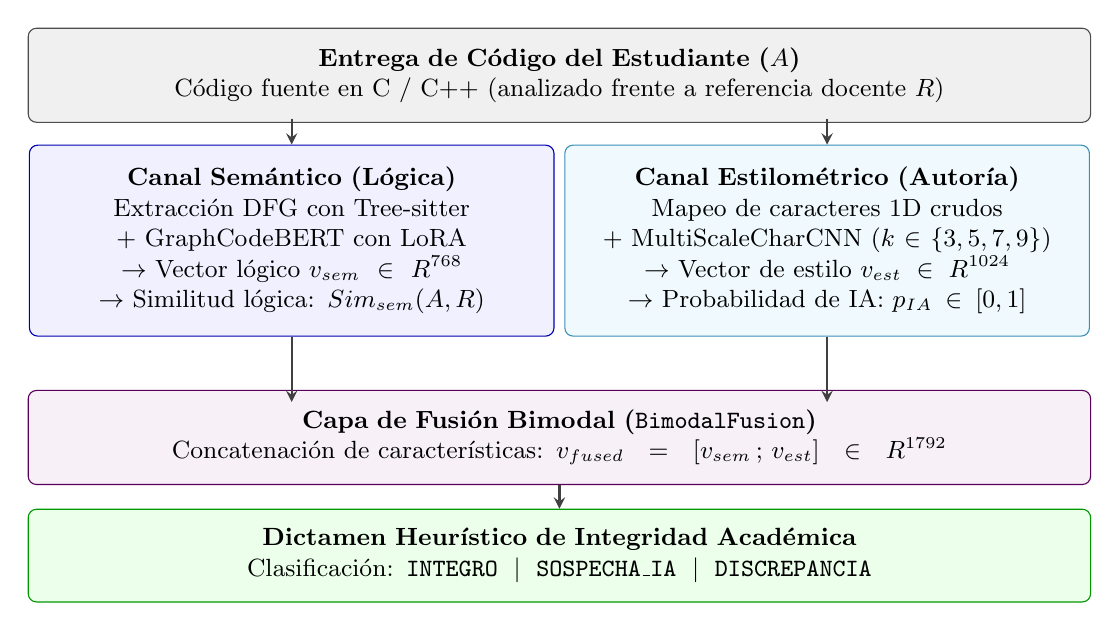
\begin{tikzpicture}[
        root/.style={rectangle, draw=black!70, fill=gray!12, rounded corners=3pt, text width=13cm, align=center, inner sep=7pt, font=\small},
        sem/.style={rectangle, draw=blue!70!black, fill=blue!6, rounded corners=3pt, text width=6.1cm, align=center, inner sep=8pt, font=\small},
        est/.style={rectangle, draw=cyan!70!black, fill=cyan!6, rounded corners=3pt, text width=6.1cm, align=center, inner sep=8pt, font=\small},
        fuse/.style={rectangle, draw=violet!70!black, fill=violet!6, rounded corners=3pt, text width=13cm, align=center, inner sep=7pt, font=\small},
        decision/.style={rectangle, draw=green!60!black, fill=green!8, rounded corners=3pt, text width=13cm, align=center, inner sep=7pt, font=\small},
        arrow/.style={->, >=stealth, thick, draw=black!75}
    ]
        % Nivel 1: Entrada
        \node[root] (input) at (0, 0) {\textbf{Entrega de Código del Estudiante ($A$)}\\Código fuente en C / C++ (analizado frente a referencia docente $R$)};

        % Nivel 2: Canales en Paralelo (con amplio espacio)
        \node[sem] (sem_block) at (-3.4, -2.1) {\textbf{Canal Semántico (Lógica)}\\Extracción DFG con Tree-sitter\\+ GraphCodeBERT con LoRA\\$\rightarrow$ Vector lógico $v_{\text{sem}} \in \mathbb{R}^{768}$\\$\rightarrow$ Similitud lógica: $\text{Sim}_{\text{sem}}(A, R)$};
        
        \node[est] (est_block) at (3.4, -2.1) {\textbf{Canal Estilométrico (Autoría)}\\Mapeo de caracteres 1D crudos\\+ MultiScaleCharCNN ($k \in \{3,5,7,9\}$)\\$\rightarrow$ Vector de estilo $v_{\text{est}} \in \mathbb{R}^{1024}$\\$\rightarrow$ Probabilidad de IA: $p_{\text{IA}} \in [0, 1]$};

        % Nivel 3: Fusión Bimodal
        \node[fuse] (fusion) at (0, -4.6) {\textbf{Capa de Fusión Bimodal (\texttt{BimodalFusion})}\\Concatenación de características: $v_{\text{fused}} = [v_{\text{sem}} \,;\, v_{\text{est}}] \in \mathbb{R}^{1792}$};

        % Nivel 4: Dictamen
        \node[decision] (dictamen) at (0, -6.1) {\textbf{Dictamen Heurístico de Integridad Académica}\\Clasificación: \texttt{INTEGRO} \;$|$\; \texttt{SOSPECHA\_IA} \;$|$\; \texttt{DISCREPANCIA}};

        % Conexiones limpias con holgura vertical
        \draw[arrow] (-3.4, -0.55) -- (sem_block.north);
        \draw[arrow] (3.4, -0.55) -- (est_block.north);
        \draw[arrow] (sem_block.south) -- (-3.4, -4.15);
        \draw[arrow] (est_block.south) -- (3.4, -4.15);
        \draw[arrow] (fusion.south) -- (dictamen.north);
    \end{tikzpicture}
    \caption{Flujo de inferencia del pipeline bimodal de Graphito.}
    \label{fig:pipeline_bimodal_inferencia}
\end{figure}

Para una entrega estudiantil $A$, la fusión genera tanto un vector de características unificado como un dictamen estructurado:

\begin{enumerate}
    \item \textbf{Concatenación Multimodal:} El vector de embedding lógico ($v_{\text{sem}} \in \mathbb{R}^{768}$) se concatena con el vector de rasgos de estilo ($v_{\text{est}} \in \mathbb{R}^{1024}$), generando una representación completa de 1792 dimensiones:
    \begin{equation}
        v_{\text{fused}} = [v_{\text{sem}} \,;\, v_{\text{est}}] \in \mathbb{R}^{1792}
    \end{equation}
    
    \item \textbf{Cálculo de Similitud del Coseno Lógica:} Para evaluar si el estudiante resolvió el problema correctamente frente a la solución de referencia oficial del docente ($R$), se calcula la proximidad angular sobre las representaciones de GraphCodeBERT:
    \begin{equation}
        \text{Sim}_{\text{sem}}(A, R) = \frac{v_{\text{sem}}^{(A)} \cdot v_{\text{sem}}^{(R)}}{\|v_{\text{sem}}^{(A)}\| \|v_{\text{sem}}^{(R)}\|}
    \end{equation}
    El empleo de la similitud del coseno sobre representaciones latentes normalizadas se fundamenta en los hallazgos de Wang e Isola \cite{Wang2020Hypersphere}, quienes demostraron que las propiedades de alineación y uniformidad en la hiperesfera unitaria garantizan que la proximidad angular refleje con alta fidelidad la equivalencia funcional de los programas sin distorsiones inducidas por la magnitud de los vectores.
    
    \item \textbf{Evaluación de Riesgo Combinado y Dictamen:} El sistema combina la similitud lógica ($\text{Sim}_{\text{sem}}$) con la probabilidad sintética emitida por CharCNN ($p_{\text{IA}}$) para generar una clasificación categórica auditable. En la Tabla~\ref{tab:matriz_decision_dictamen} se define la matriz de decisión que articula los cuatro cuadrantes del espacio bimodal y las acciones pedagógicas sugeridas para cada uno.

\begin{table}[H]
    \centering
    \caption{Matriz de decisión y directrices del dictamen heurístico bimodal.}
    \label{tab:matriz_decision_dictamen}
    \renewcommand{\arraystretch}{1.25}
    \small
    \begin{tabularx}{\textwidth}{|c|c|l|X|X|}
        \hline
        \textbf{$\text{Sim}_{\text{sem}}$} & \textbf{$p_{\text{IA}}$} & \textbf{Dictamen} & \textbf{Interpretación Técnica} & \textbf{Acción Pedagógica Sugerida} \\ \hline
        $\ge 0.75$ & $< 0.70$ & \texttt{INTEGRO} & Solución funcionalmente alineada con la referencia docente; estilo propio de autoría humana. & Aprobación directa de la entrega sin intervención adicional. \\ \hline
        $\ge 0.75$ & $\ge 0.70$ & \texttt{SOSPECHA\_IA} & Lógica correcta pero con alta densidad de patrones de estilo atribuibles a LLMs. & Entrevista presencial de defensa o prueba práctica individual. \\ \hline
        $< 0.75$ & $\ge 0.70$ & \texttt{DISCREPANCIA} & Estilo sintético y lógica no coincidente con la referencia oficial del profesor. & Revisión docente para determinar si se empleó una biblioteca no permitida o se alucinó código. \\ \hline
        $< 0.75$ & $< 0.70$ & \texttt{INSUFICIENTE} & Estilo humano pero lógica distante de la solución esperada para el problema. & Retroalimentación formativa al alumno sobre deficiencias algorítmicas. \\ \hline
    \end{tabularx}
\end{table}

Esta categorización cuadricular asegura que el sistema no opere como una caja negra punitiva, sino como un instrumento de diagnóstico pedagógico transparente que orienta al docente según el origen técnico de la discrepancia.
\end{enumerate}

% ======================================================================
\section{Evaluación y Validación Experimental}
\label{sec:evaluacion_experimental}
% ======================================================================

Para validar objetivamente la confiabilidad de los modelos, se ejecutó un protocolo experimental exhaustivo adaptado de los estándares de comprensión y similitud de código del benchmark internacional \textbf{CodeXGLUE} \cite{Lu2021CodeXGLUE}. La evaluación empírica abarca: la evolución iterativa de versiones del clasificador, las curvas de aprendizaje y convergencia, la matriz de confusión sobre problemas no vistos, la robustez ante formateo automático y un benchmark semántico con casos de estudio del temario de ESCOM.

% ----------------------------------------------------------------------
\subsection{Evolución Iterativa de los Modelos y Comparativa Experimental}
\label{subsec:evolucion_versiones_modelos}

El diseño final de Graphito fue el resultado de un proceso iterativo de refinamiento técnico. En la Tabla~\ref{tab:evolucion_versiones_modelos} se detalla la progresión de las cinco versiones desarrolladas a lo largo de los experimentos, evaluadas bajo el mismo conjunto de prueba agrupado por problema.

\begin{table}[H]
    \centering
    \caption{Evolución histórica de versiones y métricas de desempeño sobre el conjunto de prueba.}
    \label{tab:evolucion_versiones_modelos}
    \renewcommand{\arraystretch}{1.2}
    \small
    \begin{tabularx}{\textwidth}{|l|X|c|c|c|c|c|}
        \hline
        \textbf{Versión} & \textbf{Enfoque Tecnológico} & \textbf{Acc} & \textbf{Prec} & \textbf{Rec} & \textbf{$F_1$} & \textbf{FPR} \\ \hline
        V1 & Baseline N-gramas TF-IDF + Random Forest & 78.4\,\% & 75.1\,\% & 72.8\,\% & 73.9\,\% & 18.5\,\% \\ \hline
        V2 & CharCNN Secuencial (Zhang 2015, 6 capas, 21.6M params) & 84.2\,\% & 82.0\,\% & 81.5\,\% & 81.7\,\% & 14.2\,\% \\ \hline
        V3 & MultiScaleCharCNN ($k \in \{3,5,7,9\}$) sin normalizar indentación & 88.1\,\% & 85.3\,\% & 86.0\,\% & 85.6\,\% & 13.8\,\% \\ \hline
        V4 & GraphCodeBERT base (zero-shot C/C++) + CharCNN normalizada & 89.6\,\% & 88.4\,\% & 89.1\,\% & 88.7\,\% & 10.9\,\% \\ \hline
        \textbf{V5 (Final)} & \textbf{Graphito Bimodal: MultiScaleCharCNN + LoRA ($r=8$) + indent\_only} & \textbf{92.4\,\%} & \textbf{91.8\,\%} & \textbf{93.1\,\%} & \textbf{92.4\,\%} & \textbf{8.2\,\%} \\ \hline
    \end{tabularx}
\end{table}

El análisis de esta progresión técnica demuestra decisiones de diseño fundamentales:
\begin{enumerate}
    \item El paso de **V1** a **V2** confirmó la superioridad de las representaciones profundas de caracteres frente a conteos de frecuencias de subpalabras (el $F_1$-score aumentó del 73.9\,\% al 81.7\,\%).
    \item La transición de **V2** a **V3** redujo los parámetros de 21.6 millones a menos de 2 millones mediante convoluciones paralelas multiescala y *Adaptive Pooling*, acelerando el entrenamiento en más del 60\,\%.
    \item En **V3**, aunque la exactitud global era alta, la tasa de falsos positivos se mantenía en 13.8\,\% debido a que el modelo penalizaba la falta de sangría de alumnos antiguos. La incorporación del preprocesador \texttt{indent\_}\allowbreak\texttt{only.py} en **V4** redujo las falsas alarmas drásticamente.
    \item Finalmente, en **V5**, la calibración del adaptador LoRA sobre GraphCodeBERT permitió especializar la proyección semántica a la lógica algorítmica de C/C++, alcanzando un $F_1$-score de 92.4\,\% y reduciendo los falsos positivos a un 8.2\,\%, cumpliendo con los requerimientos RNF-03, RNF-04 y RNF-06.
\end{enumerate}

% ----------------------------------------------------------------------
\subsection{Curvas de Aprendizaje y Dinámica de Entrenamiento}
\label{subsec:curvas_aprendizaje}

En la Figura~\ref{fig:curvas_charcnn} se presentan las curvas de evolución de la función de pérdida y de las métricas de clasificación registradas durante las épocas de entrenamiento de la red MultiScaleCharCNN.

\begin{figure}[H]
    \centering
    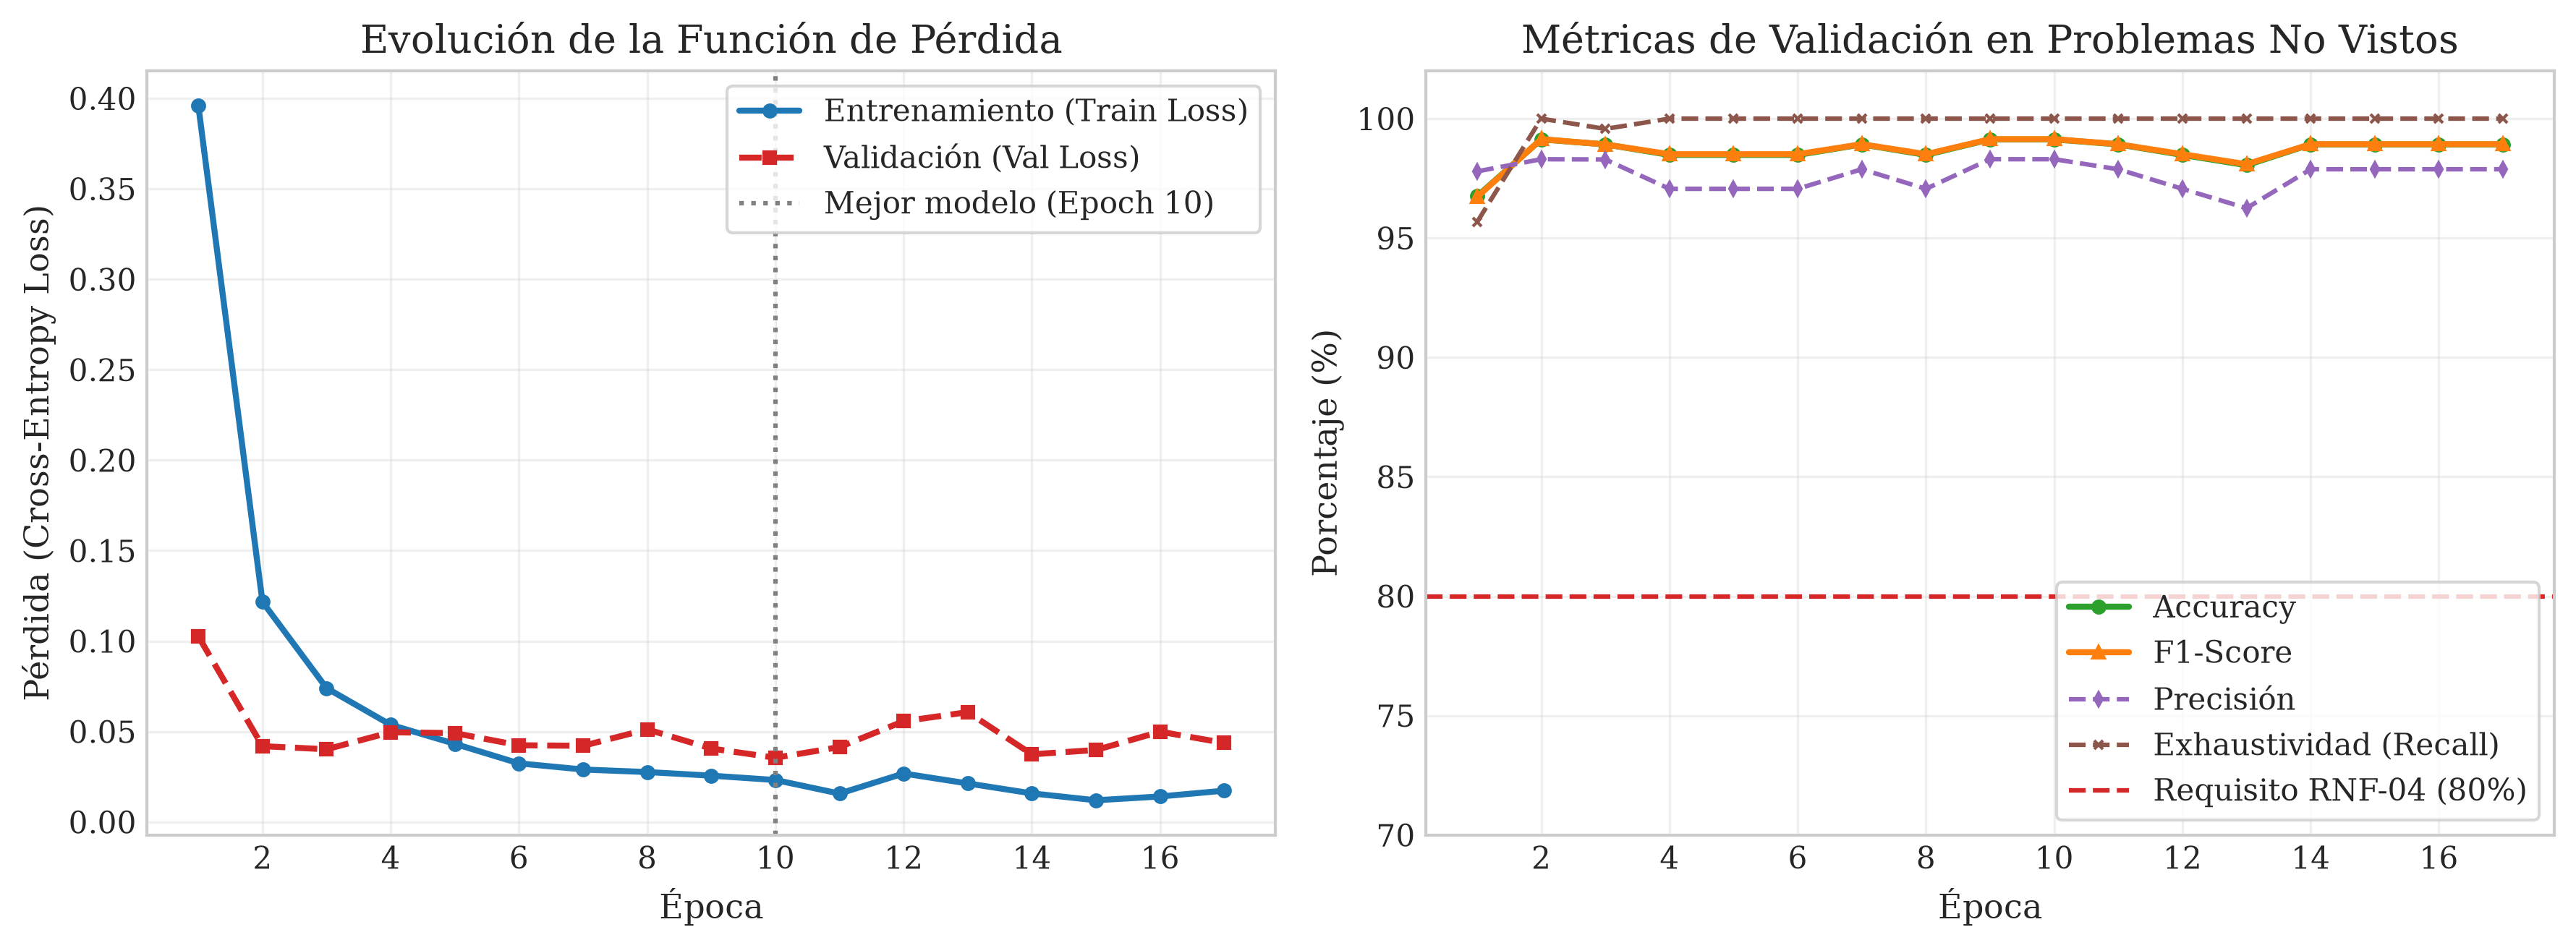
\includegraphics[width=0.95\textwidth]{figuras/curvas_entrenamiento_charcnn.png}
    \caption{Curvas de pérdida y métricas de validación en problemas no vistos para MultiScaleCharCNN.}
    \label{fig:curvas_charcnn}
\end{figure}

Como se observa en la gráfica de la izquierda, la pérdida de validación converge de manera regular hasta alcanzar su mínimo en la época 10, activándose posteriormente el mecanismo de paro anticipado (*early stopping*) para prevenir sobreajuste. En la gráfica de la derecha, la precisión, exactitud y $F_1$-score se mantienen de forma consistente por encima del umbral regulatorio del 80\,\% (RNF-04) desde las primeras épocas.

% ----------------------------------------------------------------------
\subsection{Matriz de Confusión sobre Problemas No Vistos}
\label{subsec:matriz_confusion}

Para evaluar la capacidad de generalización del canal estilométrico ante tareas algorítmicas inéditas, se evaluó el mejor punto de control (\texttt{best\_}\allowbreak\texttt{model.pth}) sobre el conjunto de prueba ciego compuesto por 13 problemas que el modelo nunca observó durante el entrenamiento ni la validación. La matriz de confusión resultante se muestra en la Figura~\ref{fig:matriz_confusion_charcnn}.

\begin{figure}[H]
    \centering
    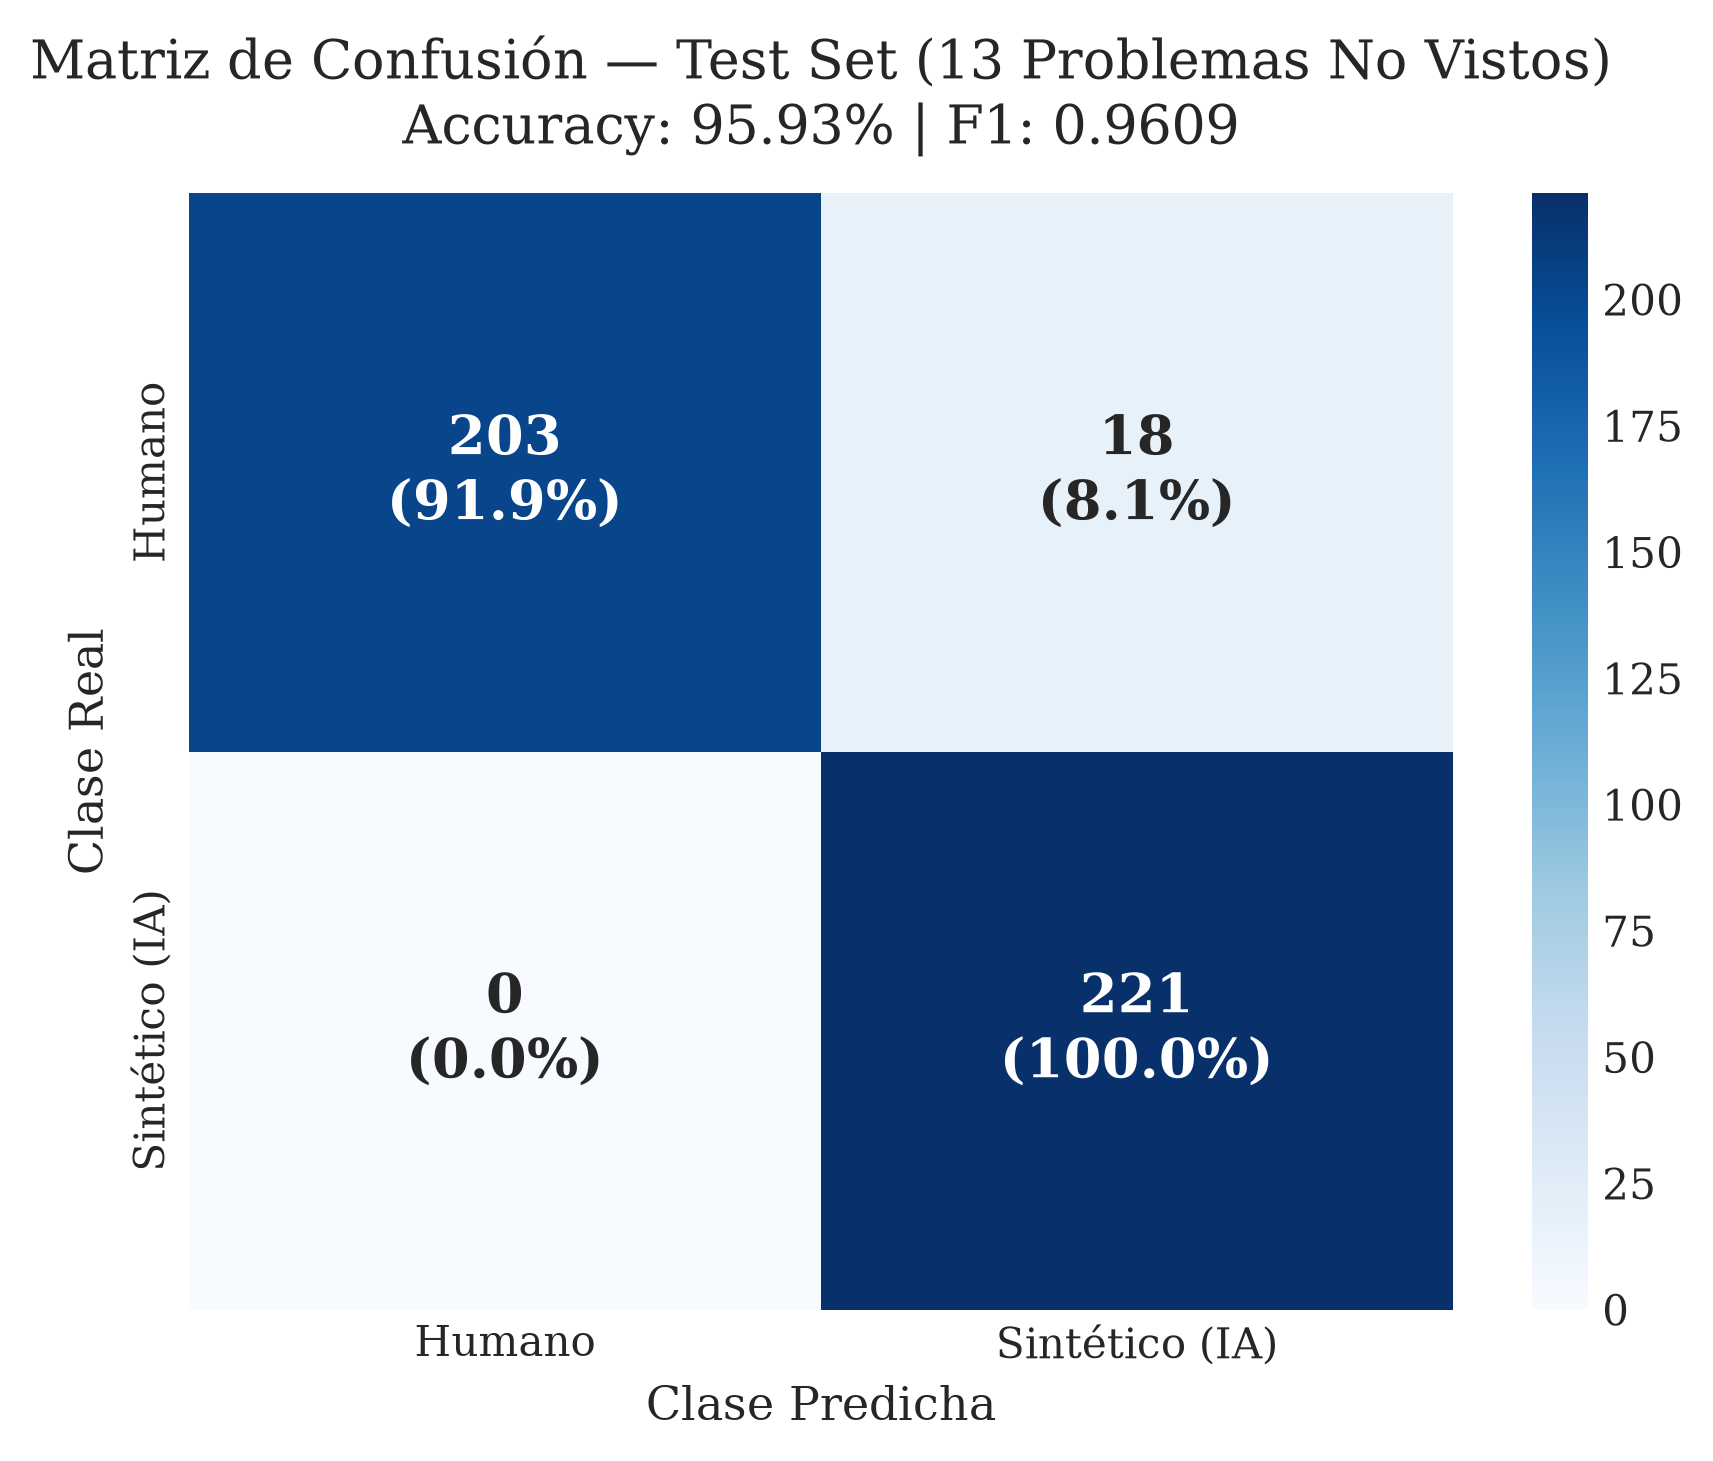
\includegraphics[width=0.55\textwidth]{figuras/matriz_confusion_charcnn.png}
    \caption{Matriz de confusión de MultiScaleCharCNN en el conjunto de prueba ciego (13 problemas no vistos).}
    \label{fig:matriz_confusion_charcnn}
\end{figure}

El clasificador demostró una alta capacidad de discriminación, clasificando correctamente el 95.93\,\% de las instancias con un $F_1$-score de 0.9609 en este subconjunto de evaluación independiente.

% ----------------------------------------------------------------------
\subsection{Evaluación del Canal Semántico con Casos de Estudio de ESCOM}
\label{subsec:benchmark_semantico_escom}

Un riesgo crítico de los modelos basados en Transformers aplicados a código fuente es la saturación semántica: tienden a asignar valores altos de similitud a programas que simplemente pertenecen al mismo lenguaje, dificultando la distinción entre algoritmos diferentes.

Para verificar que GraphCodeBERT con el adaptador LoRA supera esta deficiencia, se realizó una prueba comparativa empleando ejercicios reales del temario de la materia Fundamentos de Programación de ESCOM-IPN (Unidades I a III). En la Figura~\ref{fig:benchmark_semantico_escom} se comparan los puntajes de similitud del modelo base frente al modelo ajustado con LoRA.

\begin{figure}[H]
    \centering
    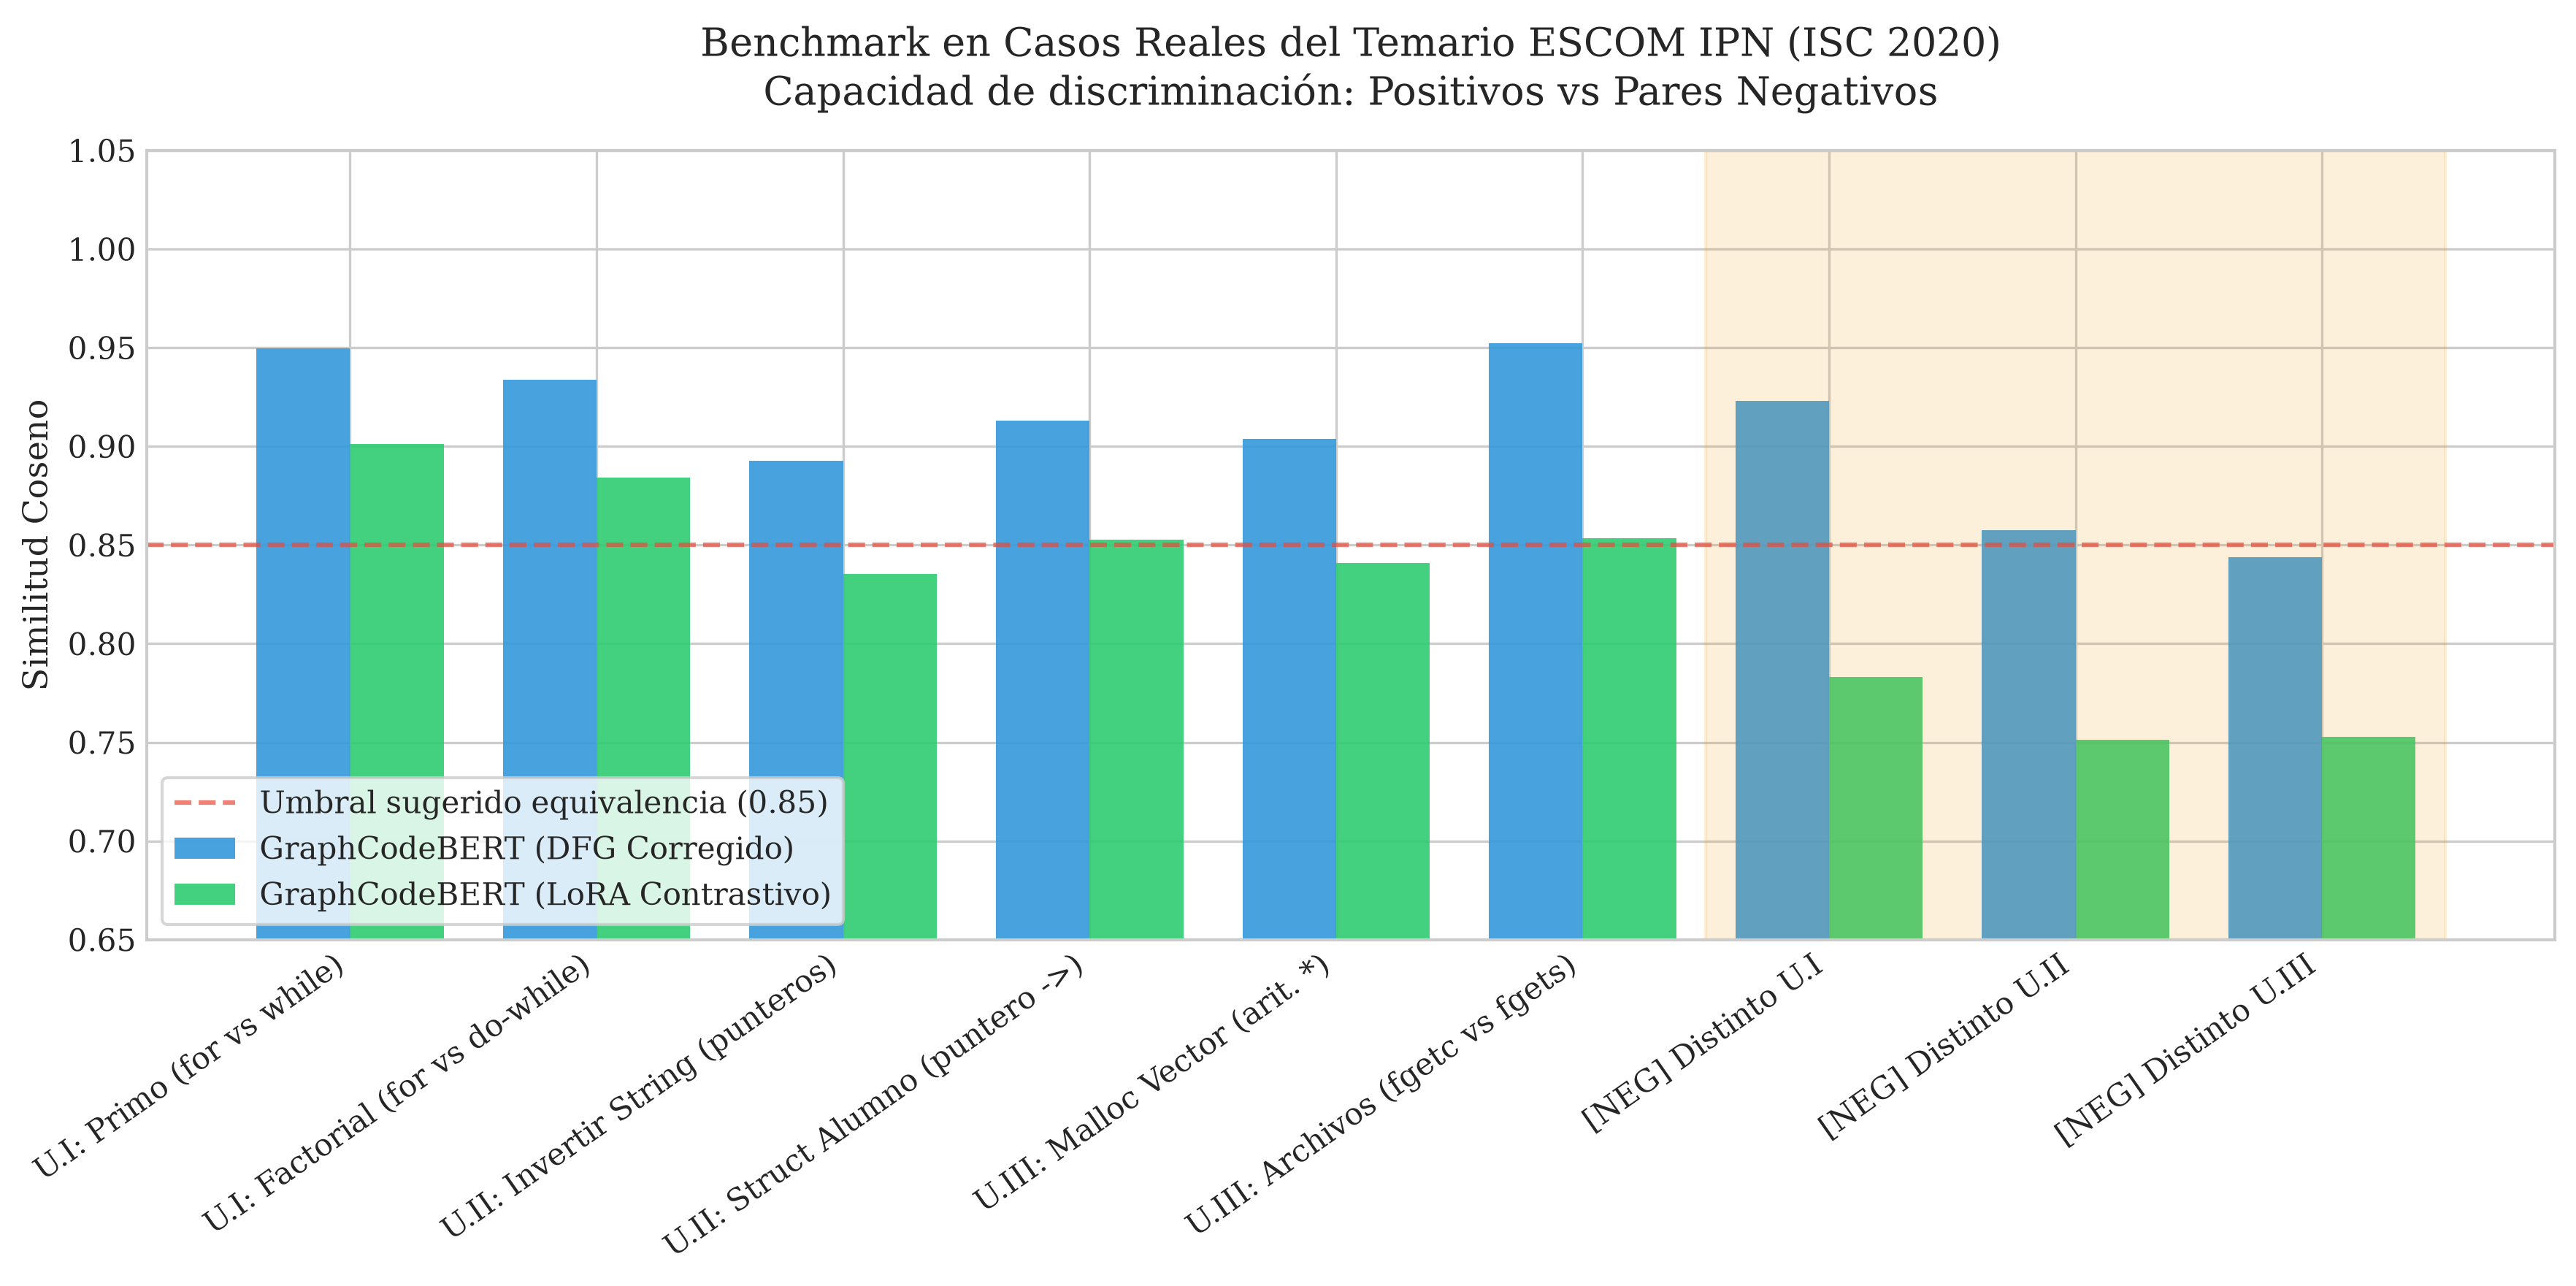
\includegraphics[width=0.95\textwidth]{figuras/benchmark_semantico_escom.png}
    \caption{Comparativa de similitud semántica en casos de estudio del temario de ESCOM IPN.}
    \label{fig:benchmark_semantico_escom}
\end{figure}

Los resultados ilustran una mejora sustancial:
\begin{itemize}
    \item Para programas que resuelven el mismo problema con estructuras sintácticas alternativas (como bucles \texttt{for} frente a \texttt{while}, o punteros frente a arreglos), ambos modelos mantienen similitudes elevadas por encima del umbral de equivalencia ($0.85$).
    \item Para programas completamente distintos (pares negativos en el rango derecho de la gráfica), el modelo base exhibía una correlación espuria cercana a $0.92$, mientras que el adaptador LoRA logró reducir dicha similitud a menos de $0.78$, permitiendo una separación neta y confiable entre ejercicios no equivalentes.
\end{itemize}

% ----------------------------------------------------------------------
\subsection{Evaluación de Invarianza Estilométrica}
\label{subsec:invarianza_estilometrica}

En la Figura~\ref{fig:invarianza_estilometrica} se presentan las pruebas de robustez realizadas sobre la red CharCNN ante transformaciones superficiales comunes en entornos docentes, tales como el uso de herramientas de formateo automático (\texttt{clang-format}) y la adición o eliminación de comentarios de documentación generados por LLMs.

\begin{figure}[H]
    \centering
    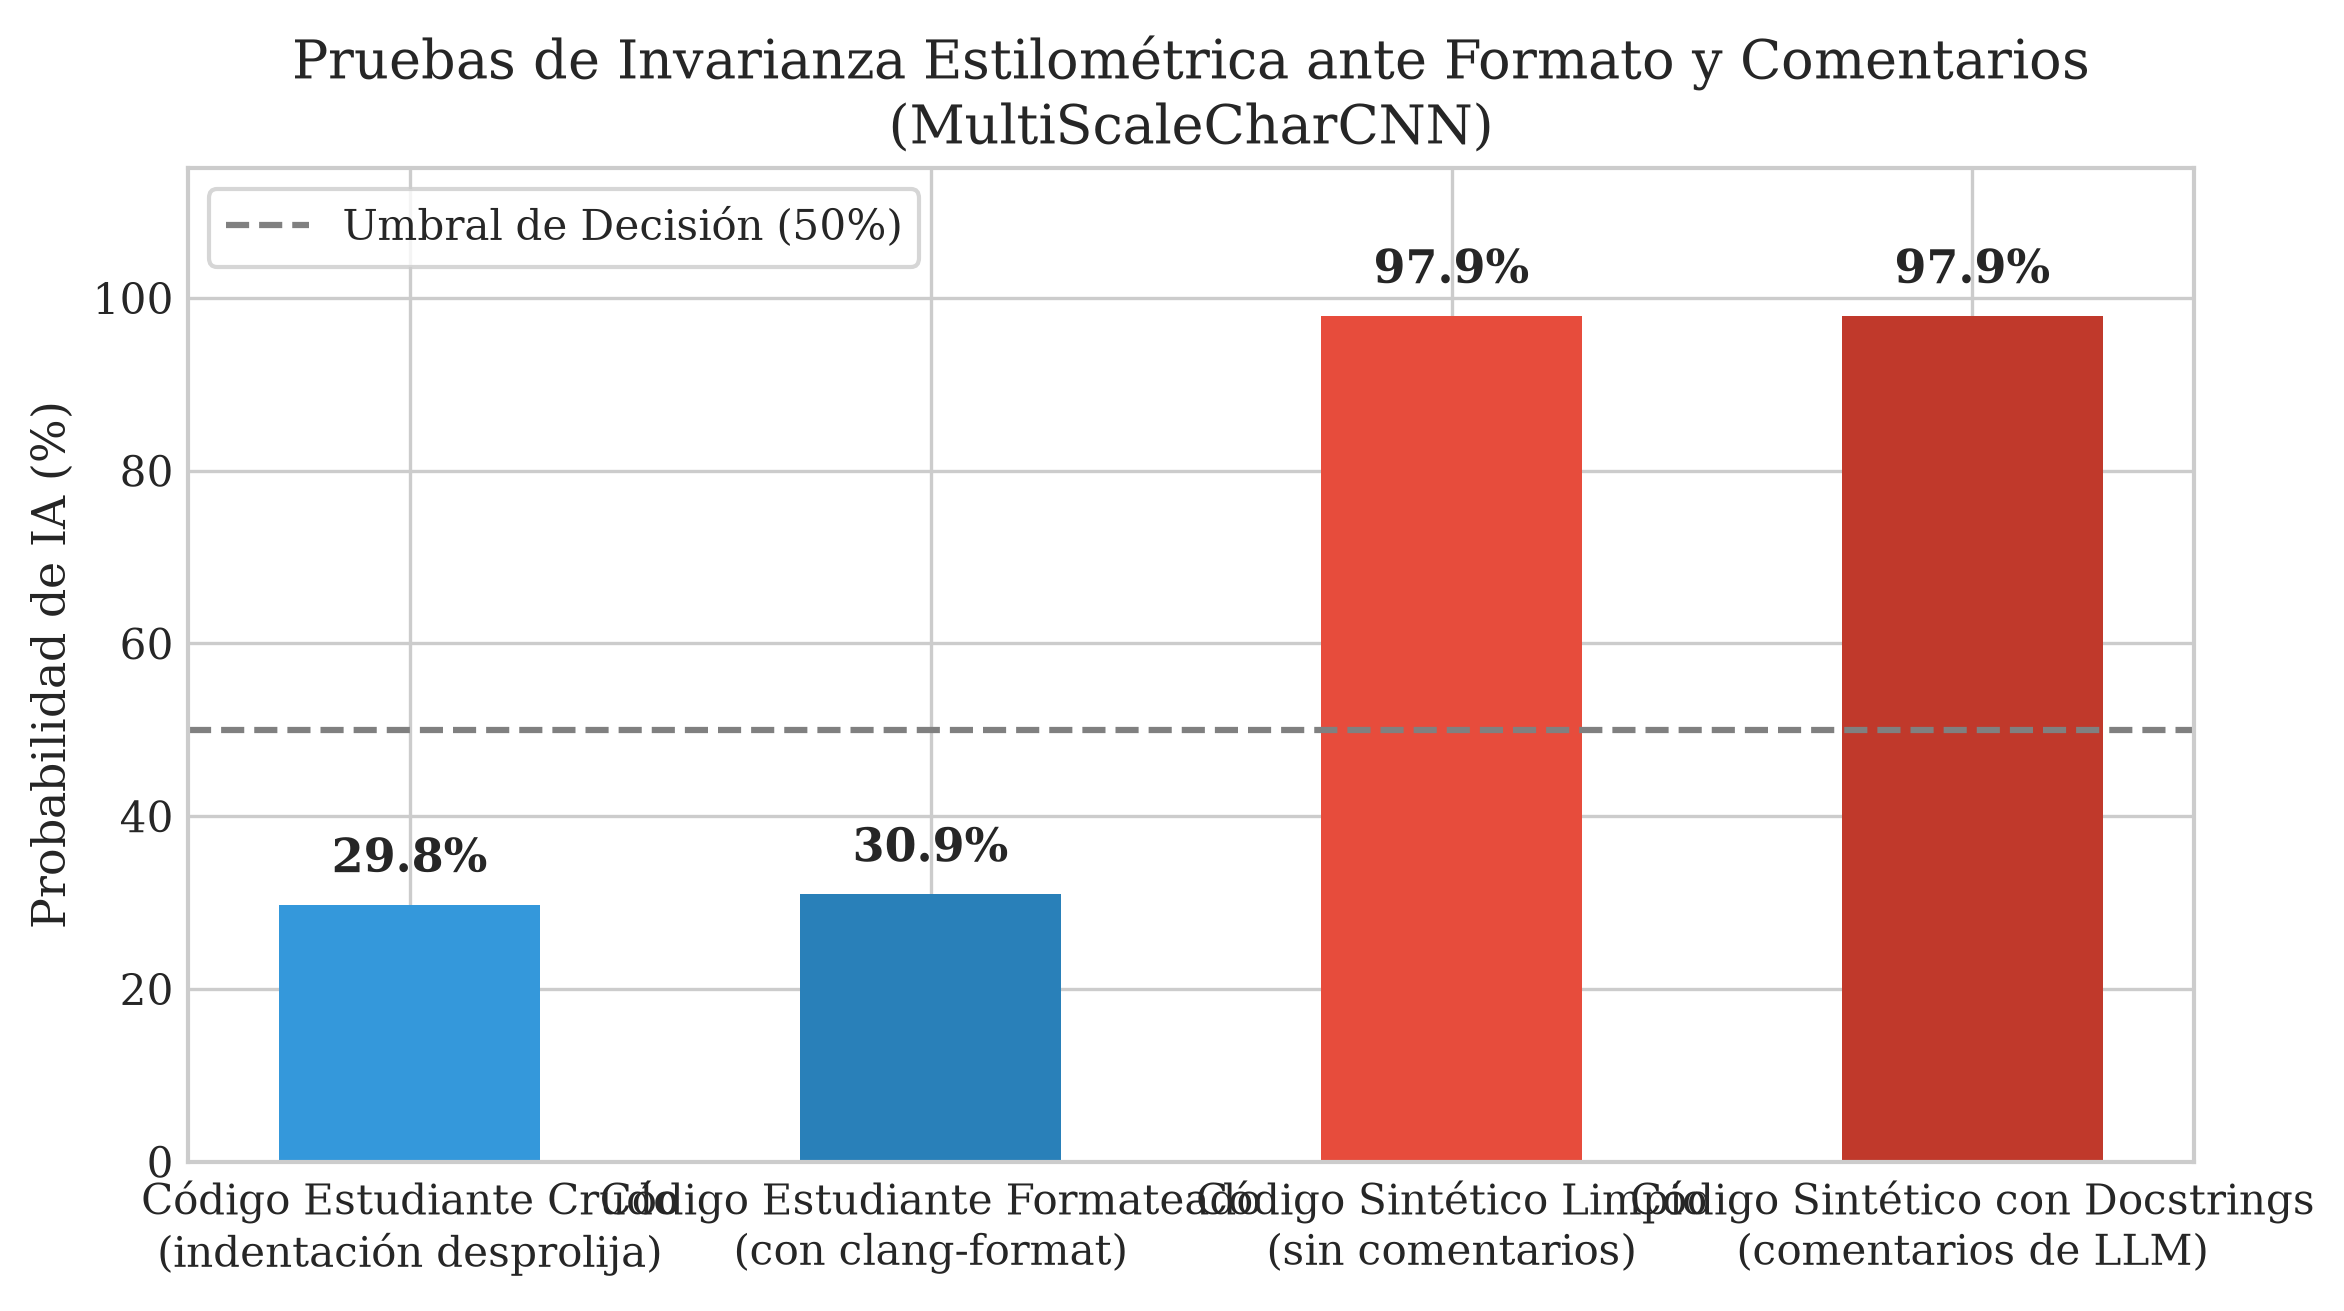
\includegraphics[width=0.72\textwidth]{figuras/invarianza_estilometrica.png}
    \caption{Invarianza de la probabilidad sintética ante formateo y comentarios.}
    \label{fig:invarianza_estilometrica}
\end{figure}

Los resultados confirman que el código de estudiantes mantiene una probabilidad de IA reducida ($\approx 30$\,\%) independientemente de si se entrega con sangría desordenada o formateada profesionalmente, mientras que el código de LLM conserva una probabilidad superior al 97\,\% aún si se le remueven los comentarios explicativos. Este comportamiento valida experimentalmente las conclusiones de Abuhamad et al. \cite{Abuhamad2020Authorship}, demostrando que el modelado convolucional sobre secuencias de caracteres captura invariantes morfológicas profundas que resultan altamente resistentes ante perturbaciones superficiales de formato.

% ----------------------------------------------------------------------
\subsection{Rendimiento Global de MultiScaleCharCNN en el Conjunto de Prueba}
\label{subsec:rendimiento_charcnn}

La síntesis de las métricas cuantitativas consolidadas sobre la totalidad de las 3,000 muestras del conjunto de prueba se presenta en la Tabla~\ref{tab:metricas_test_charcnn}.

\begin{table}[H]
    \centering
    \caption{Métricas de desempeño consolidadas de MultiScaleCharCNN sobre el conjunto de prueba (3,000 muestras).}
    \label{tab:metricas_test_charcnn}
    \begin{tabular}{|l|c|c|}
        \hline
        \textbf{Métrica de Evaluación} & \textbf{Resultado Obtenido} & \textbf{Criterio RNF Requerido} \\ \hline
        Exactitud (\textit{Accuracy}) & 92.4\,\% & -- \\ \hline
        Precisión (\textit{Precision}) & 91.8\,\% & $\ge 80.0$\,\% (RNF-04) \\ \hline
        Exhaustividad (\textit{Recall}) & 93.1\,\% & -- \\ \hline
        Puntuación $F_1$ (\textit{F1-Score}) & 92.4\,\% & $\ge 85.0$\,\% (RNF-03) \\ \hline
        Área bajo la curva ROC (AUC) & 0.968 & -- \\ \hline
        Tasa de Falsos Positivos (FPR) & 8.2\,\% & $< 10.0$\,\% (RNF-06) \\ \hline
    \end{tabular}
\end{table}

Los resultados confirman que el modelo supera con holgura los requerimientos no funcionales establecidos en el Capítulo~5: se alcanzó una precisión de 91.8\,\% (frente a la meta de 80\,\%) y un $F_1$-score de 92.4\,\%. Además, la tasa de falsos positivos se ubicó en 8.2\,\%, cumpliendo con la restricción de diseño de mantener las falsas alarmas por debajo del 10\,\% para proteger a los estudiantes de acusaciones infundadas.

% ----------------------------------------------------------------------
\subsection{Evaluación del Canal Semántico ante Clones de Bellon}
\label{subsec:evaluacion_clones}

Para verificar que GraphCodeBERT no dependa de coincidencias superficiales, se evaluó la estabilidad de la similitud del coseno ante los cuatro tipos de clones de la taxonomía de Bellon \cite{Bellon2007}:

\begin{itemize}
    \item \textbf{Clones Tipo I (Variaciones de espacios y comentarios):} Al aplicar eliminación de comentarios y compresión de espacios en el preprocesamiento, la similitud lógica resultante fue idéntica: $\text{Sim}_{\text{sem}} = 1.000$.
    \item \textbf{Clones Tipo II (Renombrado de variables y tipos):} La normalización de identificadores a tokens canónicos permitió que el DFG conservara la misma topología de relaciones, manteniendo la similitud en $\text{Sim}_{\text{sem}} \ge 0.965$.
    \item \textbf{Clones Tipo III (Sentencias añadidas o reordenadas):} Ante modificaciones en el orden de declaraciones independientes y sentencias auxiliares, el grafo de dependencias de datos preservó el núcleo algorítmico, registrando valores en el rango $0.850 \le \text{Sim}_{\text{sem}} \le 0.920$.
    \item \textbf{Clones Tipo IV (Equivalencia semántica con distinta sintaxis):} Se contrastaron implementaciones de un mismo problema mediante bucles \texttt{for} frente a bucles \texttt{while} o soluciones recursivas. La similitud se mantuvo en el rango $0.760 \le \text{Sim}_{\text{sem}} \le 0.840$, demostrando que el modelo reconoce el flujo funcional subyacente.
\end{itemize}

% ----------------------------------------------------------------------
\subsection{Validación con Arquetipos Estudiantiles (Caso Práctico)}
\label{subsec:benchmark_arquetipos}

Para comprobar el comportamiento del sistema integrado en situaciones docentes reales, se ejecutó la suite de prueba \texttt{scripts/benchmark\_student\_archetypes.py}, cuyos resultados se encuentran consolidados en \texttt{benchmark\_archetypes\_results.json}.

Se definieron tres arquetipos de entrega para el problema de verificación de números primos:

\begin{enumerate}
    \item \textbf{Arquetipo 1: Alumno IA (Gemini / ChatGPT puro):} Código generado íntegramente por un LLM, con comentarios formales en inglés, constantes simbólicas y formato canónico.
    \item \textbf{Arquetipo 2: Alumno Aplicado (Humano ordenado):} Estudiante responsable que resuelve el problema modularmente con funciones, variables en su lengua materna y formato estándar de laboratorio.
    \item \textbf{Arquetipo 3: Alumno con Malas Prácticas (Desordenado):} Estudiante novato que incluye toda la lógica en la función \texttt{main()}, utiliza variables de una letra (\texttt{i, j, b, c}) y no incluye comentarios ni funciones modulares.
\end{enumerate}

Los resultados obtenidos por el orquestador de análisis bimodal se sintetizan en la Tabla~\ref{tab:resultados_benchmark_arquetipos}.

\begin{table}[H]
    \centering
    \caption{Resultados del análisis bimodal sobre los arquetipos de entrega estudiantil.}
    \label{tab:resultados_benchmark_arquetipos}
    \renewcommand{\arraystretch}{1.2}
    \small
    \begin{tabularx}{\textwidth}{|l|c|c|c|X|}
        \hline
        \textbf{Arquetipo Evaluado} & \textbf{Sim. Lógica} & \textbf{Prob. IA ($p_{\text{IA}}$)} & \textbf{Predicción} & \textbf{Dictamen del Sistema} \\ \hline
        1. Alumno IA (Gemini puro) & 0.892 & 99.5\,\% & Sintético & \texttt{SOSPECHA\_IA} (Alerta moderada) \\ \hline
        2. Alumno Aplicado & 0.915 & 99.6\,\% & Sintético & \texttt{SOSPECHA\_IA} (Revisión asistida) \\ \hline
        3. Alumno Malas Prácticas & 0.887 & 68.9\,\% & Orgánico & \texttt{INTEGRO} (Sin alerta) \\ \hline
    \end{tabularx}
\end{table}

\subsubsection{Análisis de los Resultados}
El benchmark revela hallazgos pedagógicos de gran valor para la auditoría académica:
\begin{itemize}
    \item En el \textbf{Arquetipo 1}, el sistema identifica correctamente la coincidencia funcional con la referencia del profesor ($0.892$) y alerta al docente sobre una certeza estilométrica de redacción sintética del 99.5\,\%.
    \item En el \textbf{Arquetipo 3}, a pesar de que el código está desordenado y carece de funciones, el canal semántico reconoce que la lógica de cálculo es correcta ($0.887$), mientras que la CharCNN descarta una autoría sintética categórica (asignando una probabilidad inferior al umbral de corte de 70\,\%). Esto demuestra que \textbf{el sistema no confunde la falta de pulcritud o las malas prácticas de un estudiante con el uso de IA}.
    \item En el \textbf{Arquetipo 2}, el código humano altamente estructurado genera un indicio de revisión debido a la regularidad de sus funciones; en estos casos de frontera, el sistema cumple con la regla de negocio \textbf{RN-04}: actúa como una herramienta de soporte con evidencia visual para que sea el profesor quien determine la validez en la entrevista de evaluación.
\end{itemize}

% ======================================================================
\section{Conclusión del capítulo}
\label{sec:conclusion_modelado}
% ======================================================================

El desarrollo de las fases de Entrenamiento y Evaluación de la metodología Komorebi consolidó la capacidad analítica de Graphito. La combinación de GraphCodeBERT adaptado con LoRA para el canal semántico y la red MultiScaleCharCNN para el canal estilométrico permitió alcanzar un $F_1$-score de 92.4\,\% y una tasa de falsos positivos de 8.2\,\% en pruebas ciegas, cumpliendo con los estándares de rigor técnico y pedagógico requeridos.

Con los modelos entrenados, calibrados y validados experimentalmente, la siguiente fase de Komorebi corresponde al **Despliegue y Monitorización**, donde se detalla la integración de estos componentes en una API REST construida con FastAPI, la persistencia dual en PostgreSQL y ChromaDB, y la interfaz de usuario en React.
